\documentclass[12pt]{article}

% Language setting
\usepackage[macedonian]{babel}
\addto\captionsmacedonian{\renewcommand*\abstractname{Апстракт}}
\addto\captionsmacedonian{\renewcommand*\lstlistingname{Програмски код}}
\addto\captionsmacedonian{\renewcommand*\lstlistlistingname{Листа на програмски кодови}}
% Set page size and margins
% Replace `letterpaper' with `a4paper' for UK/EU standard size
\usepackage[a4paper,top=2cm,bottom=2cm,left=3cm,right=3cm,marginparwidth=1.75cm]{geometry}

% Useful packages
\usepackage{setspace}
\usepackage{amsmath}
\usepackage{amsfonts}
\usepackage{graphicx}
\usepackage[colorlinks=true, allcolors=black]{hyperref}
\usepackage[
    left = \flqq{},%
    right = \frqq{},%
    leftsub = \flq{},%
    rightsub = \frq{} %
]{dirtytalk}
\usepackage[font=small,labelfont=bf]{caption}
\usepackage{listings}
\usepackage{xurl}

\numberwithin{equation}{section}

% Keywords command
\providecommand{\keywords}[1]
{
  \small
  \textbf{\textit{Клучни зборови---}} #1
}

\title{Употреба на \textit{a posteriori} распределбата на сезоналните параметри во долги временски серии како \textit{a priori} распределба на сезоналните параметри во кратки временски серии}
\author{Јован Крајевски, Билјана Тојтовска}

\begin{document}
\maketitle

\newpage

\begin{abstract}
При моделирање на една популација врз основа на даден примерок, фреквенционистичката статистика се соочува со потешкотии да расуди кои статистички карактеристики на примерокот произлегуваат од популацијата, а кои произлегуваат од шумот или недоволната репрезентативност на податоците. Теоретски, Бајесовата статистика ги надминува овие потешкотии воведувајќи информирани \textit{a priori} верувања кои произлегуваат од знаењето на експертите за популацијата и кои ја ограничуваат флексибилноста на моделот да извлече заклучоци само од податоците. Во пракса, изборот на распределби кои соодветно ќе ги претстават информираните \textit{a priori} верувања не е тривијална задача. Целта на овој труд е да покаже начин информираното \textit{a priori} верување, наместо од знаењето на експертите за популацијата, да се изведе од примерок од сродна популација. Vangja, моделот кој го развивме во склоп на овој труд, е базиран на Facebook Prophet и е способен да ја искористи \textit{a posteriori} распределбата на сезоналните параметри на долги временски серии како \textit{a priori} распределба на сезоналните параметри на сродни и кратки временски серии, во кои моделирањето на сезоналноста е проблем токму поради тоа што се кратки. Моделот е тестиран на еднодимензионални берзански податоци бидејќи истите се лесно достапни, но истите техники можат да се применат и на други временски серии.
\end{abstract}

\keywords{Бајесова статистика, временски серии, FB Prophet, сезоналност, берзански податоци, PyMC, Vangja}

\newpage

\hypersetup{linkcolor=black}
\tableofcontents

\newpage

\section{Вовед}

Суштинската разлика помеѓу Бајесовата и фреквенционистичката статистика произлегува од различната интерпретација на концептот на веројатност во двете теоретски рамки. Додека фреквенционистичката статистика ја поима веројатноста како \textit{честота} на појавувањето на одреден случаен настан, Бајесовата статистика неа ја интерпретира како степен или јачина на \textit{верување} дека случајниот настан ќе се појави. Ваквата интерпретација не само што е многу поблиска до тоа како човекот ја интерпретира веројатноста, туку и ни дозволува да симулираме уште една карактеристика на човековото расудување - да ги менуваме, но не целосно, верувањата кога ќе добиеме нов примерок од популацијата.

Доколку го прифатиме Бајесовиот светоглед, тогаш примерокот од популацијата не мораме да го разгледуваме независно од нашите верувања за популацијата. Ако нашите претходни верувања за популацијата (\textit{a priori}) ги моделираме со соодветни распределби на веројатност, а потоа новите примероци од популацијата ги искористиме за да нашите \textit{a priori} верувања ги испитаме и промениме, тогаш можеме да дојдеме до нови, \textit{a posteriori} верувања. И за разлика од фреквенционистичката статистика, каде што заклучоците кои ги носиме за популацијата зависат единствено од примероците добиени од популацијата, Бајесовата статистика своите заклучоци ги носи токму од овие \textit{a posteriori} верувања, кои потекнуваат не само од примерокот, туку и од \textit{a priori} верувањата за популацијата.

Се наметнува прашањето дали и кога оваа теоретска рамка е соодветна за употреба. Сепак, статистиката тврди дека е непристрасна (или во најмала рака посакува да е непристрасна - дури и фреквенционистичката статистика посветува големо внимание на пристрасноста на своите оценувачи, но неретко се задоволува со употребата на пристрасни, но конзистентни оценувачи), а кога заклучоците за популацијата до кои статистиката пристигнува не произлегуваат исклучиво од примерокот, туку и од верувањата на статистичарот, делува дека зборуваме за нешто многу поразлично од непристрасност.

Краткиот одговор на ова прашање е едноставен. Ако примерокот е доволно голем, алатките на фреквенционистичката статистика се соодветни за употреба. Големината на примерокот до одредена мера е корелирана со репрезентативноста и непристрасноста на примерокот, како и со леснотијата да се отстрани шумот. Од друга страна, кај малите примероци е многу потешко да се зборува за репрезентативност и непристрасност. Дополнително, шумот во малите примероци е потешко да се острани без да се употребат пософистицирани методи и на тој начин да се воведе дополнителна пристрасност во понатамошната статистичка анализа. Затоа, во малите примероци каде што скоро секој пристап допушта пристрасност, алатките на Бајесовата статистика се чинат соодветни за употреба.

Но, како и повеќето кратки одговори, така и овој само површно ја обработува проблематиката. Доколку имаме голем примерок, не постои причина зошто да не се послужиме со алатките на Бајесовата статистика. Бајесовата статистика се грижи за тоа поголемите примероци да влијаат повеќе на нашите \textit{a priori} верувања и со тоа да ја намалат пристрасноста на моделот. А доколку и тоа не е доволно, секогаш можеме да ги моделираме нашите \textit{a priori} верувања со помалку информирани \textit{a priori} распределби. Големината на примерокот сама по себе не може да биде причина да не се искористи Бајесовата статистика.

И повторно, како и повеќето кратки одговори, така и овој отвара нови прашања. Како знаеме дали еден голем примерок е репрезентативен? Како знаеме дека тоа што го отстрануваме од примерокот е навистина шум? И можеби најважното прашање: колкав примерок е доволно голем примерок? Еден статистичар на последното прашање одговара со цел да покаже дека самото прашање е, во голема мера, апсурдно. Парафразирано: „Примерокот никогаш не е доволно голем, затоа што да беше доволно голем, ти сега ќе се обидуваше да решиш друг проблем за кој немаш доволно голем примерок“ \cite{never_larg}.

Прашањата кои треба да си ги поставиме за да одлучиме дали нам ни е потребно да користиме Бајесова статистика се: (1) дали поседуваме \textit{a priori} верување за популацијата кое може да ни помогне во моделирањето, и (2) дали ни е важно каква распределба има нешето \textit{a posteriori} верување за популацијата или сме задоволни со нешто поедноставно, како точкест оценувач и интервал на доверба? И само еден позитивен одговор на овие прашања значи дека треба, во најмала рака, да се погледне проблемот од перспективата на Бајесовата статистика.

Од досега изложеното може да се дојде до еден едноставен, но целосно погрешен заклучок - дека Бајесовата статистика е во секој поглед подобра од фреквенционистичката статистика. Да беше ова вистина, одамна Бајесовата статистика ќе беше почесто користена од фреквенционистичката статистика, а јасно е дека ова не е случајот. Во понатамошниот текст подробно ќе се обработат предностите и недостатоците на Бајесовата статистика, но засега мораме накратко да се осврнеме на недостатоците, бидејќи токму тие се инспирацијата зад овој труд.

Првиот недостаток е потребата од голема пресметковната моќ. Бајесовата статистика се потпира на алгоритмот Маркови Вериги Монте Карло, кој е пресметковно интензивен во однос на стандардните алгоритми кои се користат во фреквенционистичката статистика. Употребата на графички картици за паралелно процесирање, како и кај невронските мрежи, така и овде делумно го решава проблемот, но останува фактот дека невронските мрежи поседуваат многу повисок број на параметри од повеќето Бајесови модели кои се практични за употреба. Затоа и останува прашањето: чуму ми е мене Бајесов модел со \textit{N} параметри, кога во истото време, со истата пресметковна моќ, можам да истренирам невронска мрежа од \textit{10N}, \textit{100N}, \textit{1000N} параметри?

Вториот и посериозен недостаток е нејаснотијата околу методот на избор на \textit{a priori} верувањето за популацијата. Теоретски, идејата дека моделот зема предвид и \textit{a priori} верување за популацијата, дека нам ни е однапред позната одредена распределба која јасно покажува кое е нашето \textit{a priori} верување за различните „вистини“ кои ги одредуваат карактеристиките на таа популација и дека ние успешно ќе го менуваме тоа \textit{a priori} верување онака како што ќе пристигнуваат нови примероци од популацијата звучи интуитивна и едноставна за имплементација. Во пракса, проблематично е формално да ги изразиме нашите \textit{a priori} верувања за популацијата. Дури и тогаш кога тие се формални (најчесто потекнуваат од некој експерт за популацијата), преточувањето на верувања во математички распределби не е тривијална задача. Во најдобар случај, се задоволуваме со дефинирање на \textit{a priori} верувањата за популацијата добиени од некој експерт со помош на едноставни распределби, избрани бидејќи имаат убави математички својства. Во најлош случај, користиме неинформирани распределби (на пример, униформната распределба) што е занемарливо подобро од тоа воопшто да не користиме \textit{a priori} верување за популацијата.

Целта на овој труд е да покаже дека можеме да користиме информирани \textit{a priori} верувања без да се потпреме на стручноста на експертите за популацијата, конкретно во полето на временските серии. Пакетот Vangja, што го развиваме во овој труд, претпоставува дека на располагање имаме две сродни временски серии, од кои првата е доволно голем примерок од популацијата да дозволи да донесеме одредени заклучоци за нејзината сезоналност. Ваквите заклучоци, во форма на \textit{a posteriori} верување, Vangja ги искористува како \textit{a priori} верување за втората временска серија, која не е доволно голем примерок за да од нејзе изведеме заклучоци без употреба на силно информирани \textit{a priori} верувања.


\newpage

\section{Дефиниција на проблемот} \label{problem_definition}

\subsection{Неформална дефиниција}

Разгледуваме неколку временски серии - дневни типични цени на акции на берза. За секоја од овие временски серии поседуваме мал примерок од последните 3 месеци. Дополнително, на располагање имаме и временска серија од индексот на таа берза. Од оваа временска серија поседуваме голем примерок од последните 40 години. Потребно е да оцениме (предвидиме) колкава ќе е типичната цена на акциите од кои поседуваме мал примерок во наредните 365 дена.

Моделот што го користиме е Facebook Prophet \cite{taylor2018forecasting}, кој меѓу другото ни овозможува да ги моделираме и различните сезоналности во временските серии. Секоја сезоналност што сакаме да ја моделираме е дефинирана преку својата периода изразена во денови (неделната сезоналност има периода од 7 дена, годишната сезоналност има периода од 365.25 дена итн.).

Моделирајќи ги типичните цени на индекс акцијата за која поседуваме голем примерок од последните 40 години, забележуваме дека во \textit{a posteriori} верувањето е присутна силна годишна сезоналност - сезоналност која што не можеме да ја моделираме за останатите акции, бидејќи поседуваме мал примерок од последните 3 месеци. На кој начин можеме да ја искористиме моделираната \textit{a posteriori} годишна сезоналност од типичната цена на индекс акцијата за да ја моделираме годишната сезоналност на типичната цена на останатите акции?

Во понатамошниот текст, големата временската серија што ги содржи типичните цени на индекс акцијата ќе ја нарекуваме \textit{контекстна временска серија}. Малите временските серии кои ги содржат типичните цени на останатите акции ќе ги нарекуваме \textit{предиктор временски серии}.

\subsection{Формална дефиниција}

Нека е дадено множество на временски моменти (број на секунди поминати од „почетокот на времето“) \(T = (t_i : i \in \mathbb{N})\) за кои важи дека \(\forall i, j \in \mathbb{N}, i > 1, j > 1 \Rightarrow t_i - t_{i-1} = t_j - t_{j - 1} = d \) (\textbf{временските моменти се подеднакво оддалечени на растојание \(f\)}).

Нека се дадени множествата \(CT \subset T\) (\textbf{временски моменти на контекстната временска серија}), \(XT \subset T\) (\textbf{временски моменти на предиктор временските серии}) и \(FXT \subset T\) (\textbf{временски моменти за кои ги предвидуваме вредностите на предиктор временските серии}) за кои важи \(max(XT) \geq max(CT)\) (\textbf{ниту еден временски момент во \(CT\) не е во иднината, релативно на временските моменти во \(XT\)}), \( max(XT) - min(XT) = d * (\lvert XT \rvert - 1) \), \( max(CT) - min(CT) = d * (\lvert CT \rvert - 1) \), \( max(FXT) - min(FXT) = d * (\lvert FXT \rvert - 1) \) (\textbf{сите временски моменти во подмножествата се подеднакво оддалечени}) и \(min(FXT) = max(XT) + f\) (\textbf{сите временски моменти во \(FXT\) се во иднината релативно на \(XT\)}).

Нека постои непозната функција \(s: \mathbb{R} \times T \to \mathbb{R}\) за која важи \(\forall i \in \mathbb{N}, \forall p \in \mathbb{R}, i > p \Rightarrow s(p, t_i) = s(p, t_{i-p})\) (\textbf{сезоналности со периода \(p\)}). Нека се дадени и непознати функции \(f_i: \mathbb{R} \to \mathbb{R}\). Дефинираме функции \(s_i: \mathbb{R} \times T \to \mathbb{R}\) такви што

\begin{equation}\label{seasonalities_def}
  s_i(p, t) = f_i(s(p, t)) + \epsilon_t
\end{equation}
(\textbf{временските серии имаат „сродни“ сезоналности - непозната уникатна трансформација \(f_i\) на „заедничките“ сезоналности \(s\) искомбинирана со случаен шум \(\epsilon_t\)}).

Нека \(M \in \mathbb{N}\) и нека \(P = (p_1, p_2, ..., p_M) \subset \mathbb{R}\). Нека се дадени множествата \(S_i = (s_i(p_i, t): p_i \in P)\) (\textbf{конечен и ист број на сезоналности се јавуваат кај сите временски серии, без разлика дали временската серија е контекстна или предиктор временска серија}).

Нека постојат непознатите функции \(ts_i: T \times \mathbb{R}^M \to \mathbb{R}\). Нека е дадена контекстна временски серии \(C = (C_t: t \in CT)\) и предиктор временски серии \(X_i = (X_{i,t}: t \in XT)\) така што

\begin{equation}\label{timeseries_def}
  \begin{gathered}
C_t = ts_1(t, s_1(p_1, t), ..., s_1(p_M, t)) + \epsilon_t\\
X_{i,t} = ts_{i+1}(t, s_{i+1}(p_1, t), ..., s_{i+1}(p_M, t)) + \epsilon_t
  \end{gathered}
\end{equation}
(\textbf{временските серии се функции од временскиот момент и сезоналностите искомбинирани со случаен шум \(\epsilon_t\)}).

Нека за временските серии \(C\) и \(X_i\) важи дека \(\lvert C \rvert > 2 * max(P) > \lvert X_i \rvert\) (\textbf{во литературата често се среќава податокот дека за да моделираш сезоналност со периода \(p\), потребно е да имаш примерок со големина најмалку \(2p\); само контекстната временска серија го задоволува овој услов}).

При Бајесовото моделирањето на временската серија \(C\), множеството на сезоналности \(S_1\) го оценуваме со \(\widehat{S_1} = (\widehat{s_1}(p_i, \widehat{\theta_{1, i}}): p_i \in P)\), каде што \(\widehat{\theta_{1, i}}\) е некое множество на параметри. Како последица на Бајесовото моделирање, \(\widehat{\theta_{1, i}}\) е \textit{a posteriori} верување т.е. е случаен вектор со одредена распределба (\textbf{контекстната временска серија - \(C\) има доволно голем примерок за да успешно ги моделираме сите сезоналности}).

Потребно е да се предвидат елементите на множествата \(FX_i = (FX_{i,t}: t \in FXT)\) каде што вредностите \(FX_{i,t} = ts_{i+1}(t, S_i)\) и за кое важи \(\lvert FX \rvert > \lvert X \rvert \) (\textbf{хоризонтот што го предвидуваме е поголем од примерокот што го поседуваме од предиктор временските серии}).

На кој начин можеме да ја искористиме \textit{a posteriori} распределбата на \(\widehat{\theta_{1, i}}\) за да при моделирање на временските серии \(X_i\) ги оцениме множествата на сезоналности \(S_i, i > 1\) со \(\widehat{S_i} = (\widehat{s_i}(p_j, \widehat{\theta_{i, j}}): p_j \in P)\), каде што \(\widehat{\theta_{1, i}}\) е некое множество на параметри, притоа имајќи предвид дека \(2 * max(P) > \lvert X_i \rvert\) (\textbf{предиктор временските серии - \(X_i\) немаат доволно голем примерок за да успешно ги моделираме сите нивни сезоналности})?

За проблемот опишан во подсекцијата „Неформална дефиниција“ ќе важи \(\forall i \in \mathbb{N}, i > 1 \Rightarrow t_i - t_{i-1} = 24 * 60 * 60 \) (податоците се дневни), \(max(P) = 365.25\) (најголемата сезоналност е годишна), \(\lvert C \rvert = 40 * 365\) (контекстната временска серија има примерок од 40 години), \(\lvert X_i \rvert = 3 * 30\) (предиктор временските серии имаат примерок од 3 месеци) и \(\lvert FX \rvert = 365\) (предвидуваме 365 после последниот ден во примероците на предиктор временските серии).

\newpage

\section{Краток осврт на Бајесовата статистика}

За почеток ќа ја разгледаме стандардната форма која ја имаат повеќето проблеми кои статистиката се обидува да ги реши, како и пристапот на фреквенционистичката статистика за решавање на овие проблеми. Ќе разгледаме и едноставен проблем, кој ќе го решиме со методите на фреквенционистичката статистика. Сето ова ќе ни послужи како референтна точка во краткиот осврт кој што ќе го дадеме на Бајесовата статистика.

\subsection{Стандардна форма на проблемите во статистиката}

Секоја наука, без разлика дали е природна или општествена, во својата суштина решава ист проблем - моделира одреден \textit{аспект на реалноста}. Научниот метод не може да работи директно со аспектот на реалноста од интерес, туку мора да се задоволи со нејзините појави - \textit{феномени}, кои се конечни во квантитетот и се испреплетени со други феномени. Целта на научниот метод е, за даден природен или општествен феномен, да пронајде закони кои „доволно добро“ ќе го објаснат тој феномен. Најчесто, феноменот е „доволно добро“ објаснет кога пронајдените закони и заклучоците кои произлегуваат од тие закони се практично применливи за човекот.

Реалноста и нејзините феномени се производ на многубројни комплексни интеракции (помеѓу сложените форми, помеѓу простите форми, помеѓу сложените и простите форми, помеѓу сложените форми и нивните составни делови итн.) и предмет на константна промена. Доколку науката се задоволи само со тоа во целост да ги објасни сите овие комплексни интеракции и промени, научниот прогрес сигурно ќе згасне. Напротив, науката мора да се задоволи со воведување на одреден степен на апстракција во своите проучувања, со занемарување на одредени интеракции и промени, како би поставила појдовна точка кон нивно понатамошно проучување.

За таа цел, кога науката проучува одреден аспект на реалноста, таа создава модел на тој аспект на реалноста. Моделот е апстракција на аспектот на реалноста со која ние работиме за да продуцираме закони кои ги објаснуваат реалните феномени.

Колку ќе е таа апстракција блиска до реалноста зависи од тоа до кој стадиум на развој е дојдено конкретното поле на науката. Блискоста на таа апстракција до реалноста ќе биде измерена преку практичната применливост на моделот за човекот. Но, науката е игра на апроксимации. Затоа и оваа блискост на апстракцијата до реалноста првично мора да се апроксимира со одредени метрики и методи својствени за конкретното поле на науката која што ја моделира реалноста (одредени полиња ќе користат квантитативни методи, додека други полиња ќе користат квалитативни методи на проверка на блискоста на моделот со реалноста).

Статистиката е поле на математиката кое што директно се занимава со овој проблем на моделирање на реалноста - дотолку е тоа директно, што општиот проблем што статистиката го решава е аналоген на општиот проблем што науката го решава. Поконкретно, статистиката ги снабдува научниците со алатките кои им се потребни за моделирање на реалноста. А поради тоа што овие алатки кои статистиката ги продуцира се агностични во однос на полињата на науката во кои се користат, неретко и самите статистичари се занимаваат со моделирање, иако се неедуцирани во конкретното поле на науката во кое го прават моделирањето.

Секој проблем во статистиката започнува со претпоставката дека постои \textit{популација} (аналогно на аспект на реалноста). Од таа популација, нам ни е даден \textit{примерок} (аналогно на феномен). Статистиката креира модел и го подесува во однос на примерокот, надевајќи се дека овој модел успешно ќе ја апроксимира популацијата.

Моделирањето во статистиката најчесто опфаќа избор на распределби на веројатност за кои ние претпоставуваме дека, за дадени параметри на тие распределби, успешно ќе ја апроксимираат популацијата. Одредувањето на тие параметри во статистиката се нарекува оценување. Во процесот на оценување се употребува примерокот.

\subsection{Фреквенционистички пристап}

Основната претпоставка на фреквенционистичкиот пристап е поврзан со експериментите. Фреквенционистичката статистика претпоставува дека еден експеримент може да се изведе бесконечен број на пати. Под таква претпоставка, веројатноста одреден настан да се појави се поима како честота (\textit{фреквенција}) на појавување на тој настан (од таму и името „фреквенционистичка статистика“). Фреквенционистичката статистика оваа честота ја оценува од примерокот.

Во општ случај, претпоставуваме дека примерокот од популацијата следи одреден закон на распределба \(p(x; \theta)\) (без разлика дали станува збор за закон на распределба врз дискретни или апсолутно непрекинати случајни променливи/вектори/процеси). \(\theta\) се нарекуваат параметрите на овој закон на распределба и тие се непознати. Користејќи ги алатките на фреквенционистичката статистика, параметрите \(\theta\) се оценуваат, при што се добива оценувачот \(\widehat{\theta}\). Заклучоците кои понатаму можеме да ги правиме произлегуваат од законот за распределба \(p(x; \widehat{\theta})\).

Ретко кој труд за статистика е целосен без да го обработи познатиот проблем на фрлање паричка. Затоа и ние ќе го искористиме овој пример за поконкретно да ја доловиме суштината на фреквенционистичката статистика, а понатаму за да ги доловиме разликите помеѓу фреквенционистичката статистика и Бајесовата статистика.

Нека примерокот што го добиваме е \(\{X_1, X_2, ..., X_n\}\) - \(n\) случајни променливи кои настаните „се падна петка“ и „се падна глава“ ги пресликуваат во 1 и 0, соодветно. Тогаш, случајната променлива \(X_i\) можеме да ја моделираме користејќи Бернулиева шема со параметар \(p\) т.е. \(X_i \sim Bernoulli(p)\). Од нас се очекува да оцениме дали паричката е балансирана т.е. дали во популацијата од која што е извлечен добиениот примерок подеднакво често се појавуваат настаните „се падна петка“ и „се падна глава“. За таа цел, потребно е да го оцениме параметарот \(p\) со \(\widehat{p}\).

Еден од начините на кои тоа можеме да го направиме е преку средната вредност на примерокот што сме го добиле т.е. \(\widehat{p} = \frac{\sum_{i=1}^{n} X_i}{n}\). На тој начин, од Бернулиевата шема ќе следи дека честотата на настанот „се падна петка“ во популацијата изнесува \(\widehat{p}\) т.е. честотата на настанот „се падна петка“ во популацијата ја оценуваме со честотата на настанот „се падна петка“ во примерокот. Истото важи и за настанот „се падна глава“.

На крај, заклучокот за тоа дали паричката е балансирана или не ја изведуваме од законот на распределба \(Bernoulli(\widehat{p})\). Фреквенционистичката статистика ни нуди т.н. тестови со кои можеме да дојдеме до заклучокот, но во овој труд нема да посветиме повеќе внимание на нив.

\subsection{Бајесов пристап}

\subsubsection{Мотивација}

Бајесовата статистика може, аме не мора да ја земе претпоставката дека експериментот може да се изведе бесконечен број на пати за точна. Во случајот кога таа претпоставка не се зема за точна, станува проблематично веројатноста одреден настан да се појави да се поима како честота. Колку што се намалува бројот на изведувања на експериментот, толку потешко станува да зборуваме за честота и толку повеќе се јавува потребата од нова интерпретација. Затоа Бајесовата статистика се одлучува веројатноста да ја поима како степен или јачина на верување на статистичарот дека настанот ќе се појави.

Прво, да погледнеме еден корисен пример кој ја доловува разликата во пристапот кога се прифаќа и кога не се прифаќа претпоставката дека експериментот може да се изведе бесконечен број на пати, а потоа ќе се навратиме на примерот со фрлање на паричка.

Нека во една тегла има црни и бели топчиња (нивната распределба не ни е позната). Од теглата ќе извлекуваме топчиња без да ги враќаме. Пред да започнеме со извлекувањето, поставено ни е прашањето „колкава е веројатноста да извлечеме бело топче“. Бидејќи не поседуваме примерок, нашиот одговор е некоја веројатност \(p\) која што најверојатно сме ја избрале соодветно на нашите лични верувања за распределбата на топчињата. Некој ќе избере \(p=1\), што покажува дека таа личност верува дека сите топчиња во теглата се бели. Друг ќе избере \(p=0\), што покажува дека таа личност верува дека сите топчиња во теглата се црни. Трет ќе избере \(p=0.5\), што покажува дека таа личност верува дека во теглата има исто бели колку и црни топчиња.

Започнуваме да влечеме топчиња од теглата, без притоа да ги враќаме. После 10 извлекувања забележуваме дека сите извлечени топчиња се бели. Во тој момент, повторно ни се поставува истото прашање и имаме можност да избереме нова вредност за \(p\).

Доколку размислуваме како фреквенционисти, слично како и кај примерот со фрлањето паричка, ќе го оцениме \(p\) со средната вредност на примерокот и ќе речеме дека веројатноста да извлечеме бело топче е 1, без разлика на тоа каква вредност за \(p\) имаме изберено пред да започнеме со влечење на топчињата. Впрочем, фреквенционистичкиот статистичар речиси сигурно во ваква ситуација ќе избере нова вредност за \(p\) која што е поголема од вредноста за \(p\) што ја избрал пред да започне влечењето на топчињата. Но, при носењето на овој заклучок, важно е да не ја заборавиме претпоставката дека експериментот можеме да го изведеме бесконечен број на пати т.е. дека во теглата има бесконечно многу топчиња, па затоа тоа што веќе сме извлекле конечен број на топчиња нема влијание на распределбата на преостанатите топчиња во теглата.

Доколку, пак, размислуваме Бајесово, претпоставката дека експериментот можеме да го изведеме бесконечно многу пати т.е. дека во теглата има бесконечно многу топчиња не мораме да ја направиме. Доколку се одлучиме да претпоставиме дека во теглата има конечно многу топчиња, тогаш започнуваме да размислуваме поинаку од фреквенционистичкиот статистичар. Имено, ако сме извлекле 10 бели топчиња, бројот на бели топчиња кои преостанува во теглата го намалуваме за 10.

Попрецизно, Бајесовиот статистичар може да претпостави дека во теглата има \(n\) топчиња од кои \(w\) топчиња се бели, а \(n-w\) топчиња се црни. Бајесовиот статистичар има некое сопствено верување за вредноста на \(w\) кое е \(\widehat{w}\). Врз основа на ова верување, Бајесовиот статистичар, слично на фреквенционистичкиот статистичар, може пред да отпочне процесот на влечење на топчиња да го оцени \(p\) со \(\widehat{p} = \frac{\widehat{w}}{n}\). Но, после извлекувањето на 10 бели топчиња, Бајесовиот статистичар може да оцени дека во теглата преостануваат \(\widehat{w} - 10\) бели топчиња, па новата оценка на \(p\) може да биде \(\widehat{p} = \frac{\widehat{w} - 10}{n - 10} < \frac{\widehat{w}}{n}\). Затоа, ако верувањето на Бајесовиот статистичар на почетокот било дека веројатноста да извлечеме бело топче изнесува \(p\), повеќе не е контра-интуитивно тој да каже дека сега, после 10-те влечења на бели топчиња од теглата, веројатноста да извлечеме бело топче е намалена во однос на тоа што била пред да започнеме со влечење, бидејќи и бројот на бели топчиња во теглата е намален во однос на тоа што бил пред да започнеме со влечење.

Откако разгледавме како тоа што не мораме да ја направиме претпоставката дека експериментот можеме да го изведеме бесконечно многу пати го менува начинот на кој размислуваме за оценувањето на параметрите, се навраќаме на примерот со фрлањето паричка.

Како фреквенционистички статистичари, сега знаеме како да ја оцениме веројатноста дека при фрлање на паричката ќе се „падне петка“ - оценувачот е еднаков на честотата на „петки“ во примерокот. Ова е разумно решение на проблемот доколку сме ја фрлиле паричката многу пати. За 1000 фрлања и примерок од 700 инстанци на „се падна петка“ и 300 инстанци на „се падна глава“ можеме да дојдеме до доволно „сигурен“ заклучок дека честотата на „петки“ во популацијата е доволно блиску до 0.7.

Но, што ако сме ја фрлиле паричката 10 пати и во процесот сме добиле примерок од 6 инстанци на „се падна глава“ и 4 инстанци на „се падна петка“? Колкава е нашата „сигурност“ во тоа дека честотата на „петки“ во популацијата е 0.6? Колку сме сигурни дека не е 0.5 и дека ако ја фрлиме паричката уште 2 пати, нема соодносот да премине од 6-4 на 6-6?

Впрочем, размислувајќи фреквенционистички, ние немаме никаква оценка на тоа колку сме сигурни дека \(p\) е одредена вредност. Во примеров, ние не знаеме колкави се шансите \(p\) да е 0.5 наспроти тоа колкави се шансите \(p\) да е 0.6. Најдоброто нешто што можеме да го направиме е да конструираме интервал на доверба \([max(0, \widehat{p} - \widehat{\sigma}), min(1, \widehat{p} + \widehat{\sigma})]\) \footnote{Вредноста на \(p\) е ограничена на интервалот \([0, 1]\), па затоа и интервалот на доверба не може да лежи надвор од \([0, 1]\).} околу \(\widehat{p}\) и да кажеме дека сме \(c\%\) сигурни дека \(p\) се наоѓа во тој интервал, а \(1-c\%\) сигурни дека \(p\) се наоѓа надвор од тој интервал.

Конструкцијата на интервалот на доверба во фреквенционистичка статистика повторно се основа на претпоставката дека експериментот можеме да го изведеме бесконечно многу пати. Без разлика на тоа што во претходниот параграф низ зборевме за „сигурноста“ т.е. верувањето дека \(p\) се наоѓа во нашиот интервал на доверба, фреквенционистичката статистика не препознава таков концепт на верување. Наместо тоа, претпоставката е дека ако добиеме бесконечен број на серии на експерименти \(\{\{X_{1,1}, X_{1,2}, ..., X_{1,n_1}\}, \{X_{2,1}, X_{2,2}, ..., X_{2,n_2}\}, ...\}\), честотата со која \(p\) ќе се наоѓа во нашиот интервал со \(c\%\) доверба изнесува \(c\%\) \footnote{Проблематично е што претходно го земавме \(\widehat{p}\) за средина на интервалот на доверба. Ако постои интервал на доверба во кој во \(c\%\) од примероците ќе се наоѓа \(\widehat{p}\), тогаш шансите дека нашиот оценувач \(\widehat{p}\) воопшто не се наоѓа во тој интервал е \(1 - c\%\). За да конструираме интервал на доверба каде што \(\widehat{p}\) се наоѓа во средината на тој интервал, потребно е да се \(100\%\) „сигурни“ дека \(\widehat{p}\) се наоѓа во интервалот на доверба и дека е во средината на тој интервал. Ваква „сигурност“ немаме. Каква смисла има тогаш вака конструираниот интервал, кој можеби воопшто нема пресек со интервалот кој што ние претпоставуваме дека постои?}.

На овој начин, ефектот што се постигнува е оценувачот \(\widehat{p}\) од конкретна вредност да прерасне во случајна променлива со сопствен закон на распределба:

\[p_{\widehat{p}}(x) = \begin{cases}
    \frac{1 - c\%}{1 - (min(1, \widehat{p} + \widehat{\sigma}) - max(0, \widehat{p} - \widehat{\sigma}))} & x \notin [max(0, \widehat{p} - \widehat{\sigma}), min(1, \widehat{p} + \widehat{\sigma})] \\
    \hfil \frac{c\%}{min(1, \widehat{p} + \widehat{\sigma}) - max(0, \widehat{p} - \widehat{\sigma})} & x \in [max(0, \widehat{p} - \widehat{\sigma}), min(1, \widehat{p} + \widehat{\sigma})]
\end{cases}\]

Бајесовиот статистичар нема да се задоволи со ваков закон на распределба. Од една страна, \(p_{\widehat{p}}(x)\) препишува една иста густина на распределба на сите точки кои лежат во интервалот на доверба - \(\frac{c\%}{min(1, \widehat{p} + \widehat{\sigma}) - max(0, \widehat{p} - \widehat{\sigma})}\). Истото важи и за сите точки кои лежат надвор од интервалот на доверба, за кои повторно \(p_{\widehat{p}}(x)\) препишува една иста густина на распределба - \(\frac{1 - c\%}{1 - (min(1, \widehat{p} + \widehat{\sigma}) - max(0, \widehat{p} - \widehat{\sigma}))}\).

Од друга страна, \(p_{\widehat{p}}(x)\) е одредена единствено од примерокот што го разгледуваме. Но, што ако пред да започнеме да ја фрламе паричката, имаме некое силно верување дека паричката што ја фрламе е балансирана (можеби целта на производителот на паричката била таа да е балансирана)? Или, спротивно на тоа, што ако пред да започнеме да ја фрламе паричката, имаме некое силно верување дека паричката што ја фрламе воопшто не е балансирана и е пристрасна кон настанот „се падна глава“ (можеби целта на производителот на паричката била таа да е пристрасна кон едната страна)? Под претпоставка дека примерокот содржи 6 инстанци на „се падна глава“ и 4 инстанци на „се падна петка“, зависно од двата наши претходни верувања би требало да добиеме различна оценка за \(p\).

Во првиот случај, кога веруваме дека паричката што ја фрламе е балансирана, бајесовиот статистичар ќе се обиде ова верување да го инкорпорира во моделот на начин на кој од примерокот од 6 инстанци на „се падна глава“ и 4 инстанци на „се падна петка“ ќе оцени дека сепак веројатноста \(p\) да е 0.5 е повисока од веројатноста \(p\) да е 0.6. Во вториот случај, кога веруваме дека паричката што ја фрламе не е балансирана и е пристрасна кон случајниот настан „се падна глава“, бајесовиот статистичар ќе се обиде ова верување да го инкорпорира во моделот на начин на кој од примерокот од 6 инстанци на „се падна глава“ и 4 инстанци на „се падна петка“ ќе оцени дека веројатноста \(p\) да е 0.6 е значително повисока од веројатноста \(p\) да е 0.5.

Овие два недостатоци на фреквенционистичката статистика, да се оцени законот на распределба на параметарот што го оценуваме и да се инкорпорираат претходни верувања за параметарот што го оценуваме, се мотивацијата за развој на Бајесовата статистика.

\subsubsection{Од \textit{a priori} до \textit{a posterior}i верувања преку Бајесовата теорема}

Бајесовата статистика ги третира оценувачите на параметрите \(\theta\) како случајни променливи со сопствени закони на распределба. Во примерот со фрлањето паричка, тоа ќе значи дека не само што случајните променливи од примерокот следат одредена распределба т.е. \(X_i \sim Bernoulli(p)\), туку и оценувачот на \(p\) следи одредена распределба. Распределбата што ја следи оценувачот пред да го добиеме примерокот се нарекува \textit{a priori} верување или \textit{a priori} распределба на параметарот, а распределбата што ја следи оценувачот откако ќе го добиеме примерокот се нарекува \textit{a posteriori} верување или \textit{a posteriori} распределба на параметарот.

\textit{A priori} распределбата на параметрите ја запишуваме како \(p(\widehat{\theta})\). Наредното прашање кое треба да си го поставиме е: колкава е веројатноста даден примерок на популацијата да потекнува од дадената \textit{a priori} распределба на параметрите? Ваквата веројатност во Бајесовата статистика се нарекува подобност. Доколку го обележиме примерокот со \(X \sim \{X_1, ..., X_n\}\), подобноста можеме да ја запишеме како \(p(X|\widehat{\theta})\). Конечно, \textit{a posteriori} распределбата на параметрите можеме да ја запишеме како \(p(\widehat{\theta}|X)\).

За да ја пресметаме \textit{a posteriori} распределбата на параметрите \(p(\widehat{\theta}|X)\) за дадени \textit{a priori} распределба на параметрите \(p(\widehat{\theta})\) и примерок \(X\) ја користиме Бајесовата теорема \cite{wiki:bayes_theorem} од која следи:

\begin{equation}\label{bayes_eq}
p(\widehat{\theta}|X) = \frac{p(X|\widehat{\theta})p(\widehat{\theta})}{p(X)}
\end{equation}

Пресметката на \(p(X)\) во (\ref{bayes_eq}) не е тривијална задача, но за среќа не е ни потребна. Од интерес ни е релативниот сооднос на вредностите на оценувачот \(\theta\), додека именителот \(p(X)\) служи само за да \(p(\widehat{\theta}|X)\) ги задржи карактеристиките кои еден закон на распределба мора да ги има (ги скалира густините на распределба за нивната сума/определениот интеграл изнесува 1). Затоа, (\ref{bayes_eq}) можеме да го упростиме:

\begin{equation}\label{bayes_eq_sim}
p(\widehat{\theta}|X) \sim p(X|\widehat{\theta})p(\widehat{\theta})
\end{equation}

Да разгледаме до какви заклучоци ќе пристигнеме користејќи ја Бајесовата статистика во решавање на примерот со фрлање на паричка доколку сме претпоставиле дека паричката е пристрасна кон настанот „се падна петка“ и, спротивно на тоа, доколку сме претпоставиле дека паричката не е пристрасна. Во двата случаи ќе работиме со примерокот од 6 инстанци на „се падна глава“ и 4 инстанци на „се падна петка“.

Прво, да го погледнеме случајот кога нашата претпоставка е дека паричката е пристрасна кон настанот „се падна петка“. Оваа претпоставка значи дека ние веруваме дека распределбата на оценувачот на параметарот \(p\) е таква што веројатноста \(p\) да е поголем од 0.5 е поголема од веројатноста \(p\) да е помал од 0.5.

Математички, згодно ни е да претпоставиме дека \(\widehat{p} \sim Beta(\alpha, \beta)\). Од една страна, Бета распределбата е погодна за моделирање на \(\widehat{p}\) бидејќи е ограничена на интервалот \([0, 1]\) и бидејќи, доколку нашето \textit{a priori} верување е неинформирано и сакаме да употребиме униформна распределба за моделирање на \(\widehat{p}\), тоа повторно можеме да го направиме со Бета распределбата бидејќи \(Beta(1, 1) = Uniform(0, 1)\).

Од друга страна, Бета распределбата е посебен тип на распределба која се нарекува конјугирана распределба. Во Бајесовата статистика, конјугирана распределба е онаа распределба која, доколку ја искористиме како \textit{a priori} распределба, за одредена подобност ќе резултира во \textit{a posteriori} распределба која припаѓа на истата фамилија на распределби како и \textit{a priori} распределбата.

\begin{figure}[h]
    \centering
    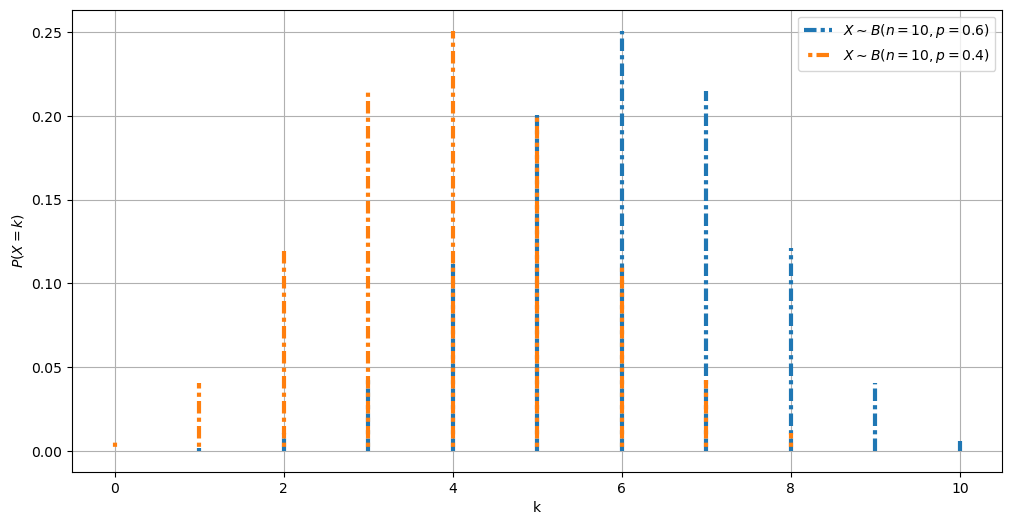
\includegraphics[width=1\textwidth]{plots/binom.png}
    \caption{Биномна распределба на подобноста за различна вредност на \(p\)}
    \label{fig:binom}
    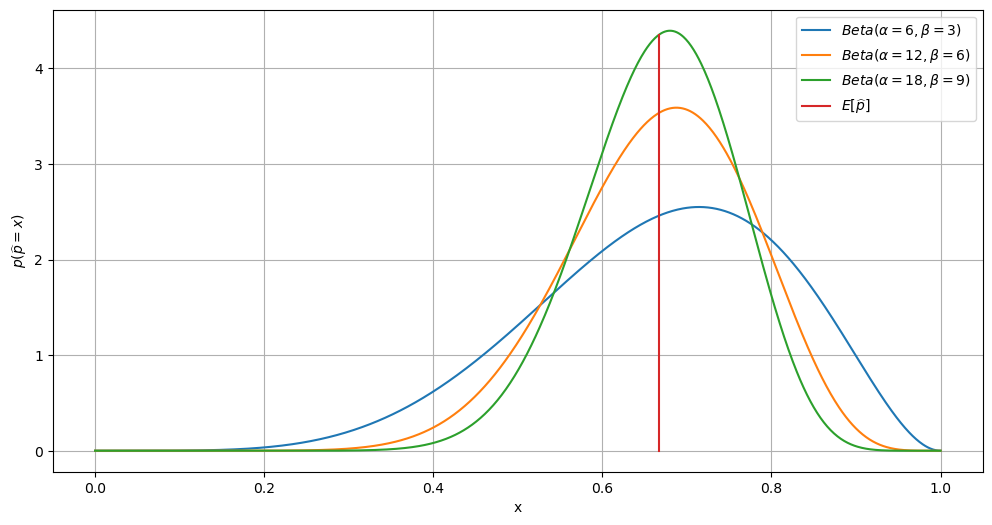
\includegraphics[width=1\textwidth]{plots/betas.png}
    \caption{Влијанието на изборот на \(\beta\) врз \textit{a priori} распределбата на \(\widehat{p}\)}
    \label{fig:betas}
\end{figure}

Бета дистрибуцијата е конјугирана распределба, доколку подобноста следи Биномна распределба \cite{wiki:conjugate_prior}. На сликата \ref{fig:binom} можеме да погледнеме различни Биномни распределби на подобноста. Забележуваме дека подобноста на примерокот што го разгледуваме (6 инстанци на „се падна глава“ и 4 инстанци на „се падна петка“) е различна за \(p=0.6\) и за \(p=0.4\) т.е. дека нашиот примерок е многу поверојатно (над 2 пати поверојатно) да потекнува од Биномна распределба со параметар \(p=0.6\) од тоа што е веројатно да потекнува од Биномна распределба со параметар \(p=0.4\).

За даден примерок \(X = \{X_1, X_2, ..., X_n\}\) каде што \(X_i \sim Bernoulli(p)\) важи:

\begin{equation}\label{conjugate_beta}
  \begin{gathered}
    X_i \sim Bernoulli(p), Y=\sum_{i=1}^{n} X_i \Rightarrow Y \sim Binomial(n, p)\\
    \widehat{p} \sim Beta(\alpha, \beta), Y \sim Binomial(n, \widehat{p}) \Rightarrow \widehat{p}|Y \sim Beta(\alpha + Y, \beta + n - Y)
  \end{gathered}
\end{equation}

Бета распредлбата има такви својства да ние можеме параметрите \(\alpha\) и \(\beta\) да ги интерпретираме како број на појавувања на настанот „се падна петка“ и број на појавувања на настанот „се падна глава“ соодветно. Од (\ref{conjugate_beta}) следи дека нашето верување за односот помеѓу веројатноста на настанот „се падна петка“ и веројатноста на настанот „се падна глава“ е еднаков на односот помеѓу \(\alpha\) и \(\beta\) т.е. \(\frac{p(\widehat{p})}{1 - p(\widehat{p})} = \frac{\alpha}{\beta}\). Доколку, на пример, нашето \textit{a priori} верување е дека е три пати поверојатно да се случи настанот „се падна петка“ од тоа да се случи настанот „се падна глава“, тогаш потребно е да избереме такви \(\alpha\) и \(\beta\) за да нивниот сооднос е 3:1 т.е. да важи \(\alpha=3\beta\).

Изборот, пак, на \(\beta\) (следствено на тоа што ни е познат соодносот помеѓу \(\alpha\) и \(\beta\)), еднозначно ја одредува и вредноста на \(\alpha\). Значењето на овој параметар се интерпретира како степен или јачината на нашето верување во односот помеѓу веројатноста на настанот „се падна петка“ и веројатноста на настанот „се падна глава“. Колку сме посигурни во тоа дека \(p(\widehat{p}) = 3(1 - p(\widehat{p}))\), толку повисока вредност на \(\beta\) треба да избереме.

На сликата \ref{fig:betas} се забележува дека изборот на поголема вредност на \(\beta\) ја намалува дисперзијата на \(\widehat{p}\) т.е. ја зголемува довербата дека \(p(\widehat{p}) = 3(1 - p(\widehat{p}))\) т.е. дека вредноста на \(\widehat{p}\) изнесува \(\frac{3}{4}\).

\begin{figure}[h]
    \centering
    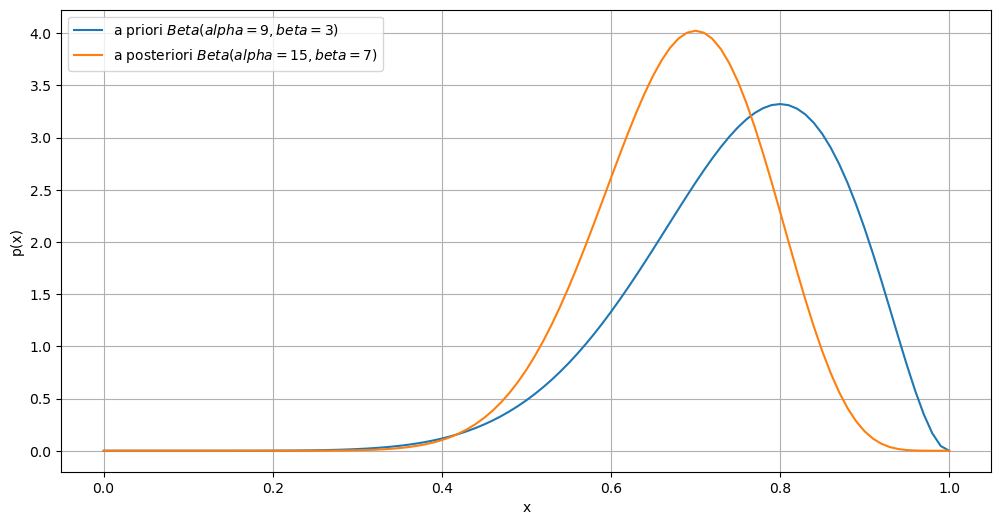
\includegraphics[width=1\textwidth]{plots/beta_prior_to_posterior.png}
    \caption{Од \textit{a priori} \(Beta(\alpha=6, \beta=3)\) до \textit{a posteriori}}
    \label{fig:beta_prior_to_posterior}
\end{figure}

Од (\ref{conjugate_beta}) е јасно како ќе изгледа \textit{a posteriori} Бета распределбата за дадена \textit{a priori} Бета распределба и подобност со Биномна распределба. Во случајот кога кај нас постои \textit{a priori} верување дека \(p(\widehat{p}) = 3(1 - p(\widehat{p}))\) и истото е моделирано со распределба \(Beta(\alpha=9, \beta=3)\), примерокот преку подобноста ја менува оваа распределба во \(Beta(\alpha=15, \beta=7)\) \textit{a posteriori} распределба во која верувањето \(p(\widehat{p} = 0.5 | X)\) e барем 4 пати пониско од верувањето \(p(\widehat{p} = \frac{15}{22} | X)\) (погледни слика \ref{fig:beta_prior_to_posterior}).

\begin{figure}[h]
    \centering
    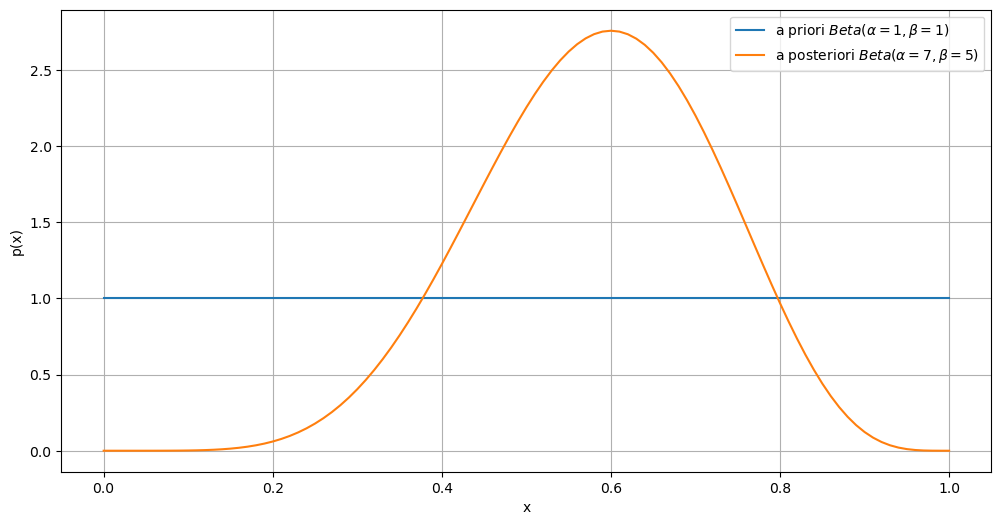
\includegraphics[width=1\textwidth]{plots/uniform_prior_to_posterior.png}
    \caption{Од \textit{a priori} \(Beta(\alpha=1, \beta=1)\) до \textit{a posteriori}}
    \label{fig:uniform_prior_to_posterior}
\end{figure}

Во случајот кога кај нас постои неинформирано \textit{a priori} верување и истото е моделирано со распределба \(Beta(\alpha=1, \beta=1) = Uniform(0, 1)\), примерокот преку подобноста ја менува оваа распределба во \(Beta(\alpha=7, \beta=5)\) \textit{a posteriori} распределба во која верувањето \(p(\widehat{p} = 0.5 | X)\) e далеку поблиску до верувањето \(p(\widehat{p} = \frac{7}{12} | X)\) (погледни слика \ref{fig:uniform_prior_to_posterior}). Од тука се забележува дека кога примерокот е мал, \textit{a priori} верувањата имаат големо влијание.

За крај покажуваме и дека поголемите примероци го намалуваат влијанието на \textit{a priori} верувањата. Да претпоставиме дека нашето \textit{a priori} верување во \(p(\widehat{p}) = 3(1 - p(\widehat{p}))\) е многу силно и истото е моделирано со распределба \(Beta(\alpha=90, \beta=30)\) (што е еквиваленто на тоа да сме сведочеле 120 фрлања на паричката, од кои 90 резултирале во настанот „се падна глава“). Нека нашиот примерок се состои од 1000 фрлања на паричката, каде што има 520 инстанци на „се падна глава“ и 480 инстанци на „се падна петка“. Примерокот преку подобноста ја менува \textit{a priori} распределбата во \(Beta(\alpha=610, \beta=510)\) \textit{a posteriori} распределба во која верувањето дека паричката е балансирана е многу високо, и покрај тоа што \textit{a priori} верувањето дека паричката е балансирано е многу мало (погледни слика \ref{fig:beta_prior_to_posterior_large}).

\begin{figure}[h]
    \centering
    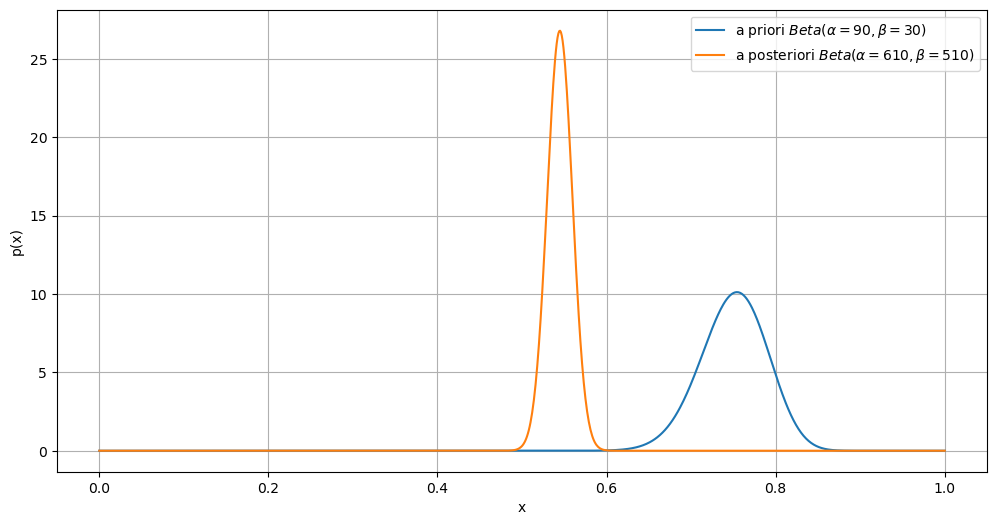
\includegraphics[width=1\textwidth]{plots/beta_prior_to_posterior_large.png}
    \caption{Од \textit{a priori} \(Beta(\alpha=90, \beta=30)\) до \textit{a posteriori} со голем примерок}
    \label{fig:beta_prior_to_posterior_large}
\end{figure}

\subsubsection{MCMC и MAP}

Нажалост, многу е тешко да се задржат убавите математички карактеристики кои ги нудат конјугираните распределби со зголемувањето на димензионалноста на моделот. Конјугираните распределби се малку во број, а нивното комбинирање речиси никогаш не резултира во нови, повеќедимензионални конјугирани распределби. Затоа, доколку одлучиме да користиме исклучиво конјугирани распределби во нашето моделирање со цел поедноставно пресметување на \textit{a posteriori} распределбата, принудени сме да не користиме голем број на параметри во моделите. Како последица, бројот на појави кои успешно ќе можеме да ги измоделираме драстично ќе се намали.

Не само што е потешко, туку и речиси е невозможно аналитички да се одреди \textit{a posteriori} распределбата на повеќедимензионални модели. Но тоа што можеме во пракса да го направиме е истите нумерички да ги апроксимираме. Постојат различни фамилии на пристапи кои можеме да ги направиме за апроксимација, но фамилијата на Маркови Вериги Монте Карло (Markov Chain Monte Carlo - MCMC) е една од најчесто користените во пракса.

Идејата на MCMC алгоритмите е да влечат примероци од \textit{a posteriori} распределбата, притоа фаворизирајќи ги оние примероци за кои \textit{a posteriori} распределбата е повисока. Во овие алгоритми најчесто дефинираме и критериум на прифаќање на извлечените примероци. Доколку извлечениот примерок е прифатен, тој примерок се додава на трасата примероци \(trace\) која служи за апроксимирање на \textit{a posteriori} распределбата и понатамошното влечење на примероци е афектирано од последниот прифатен примерок.

Заедничките чекори за повеќето различни MCMC алгоритми се следниве:

\begin{enumerate}
    \item Постави ја трасата на празна подредена торка (\(trace \leftarrow ()\))
    \item Избери целна должина \(M\) на \(trace\)
    \item Избери почетна вредност \(\widehat{\theta}_{init}\)
    \item Постави ја сегашната вредност на почетната вредност (\(\widehat{\theta}_{current} \leftarrow \widehat{\theta}_{init}\))
    \item Пресметај ја релативната \textit{a posteriori} распределба на сегашната вредност \(p(X|\widehat{\theta} = \widehat{\theta}_{current})p(\widehat{\theta} = \widehat{\theta}_{current})\)
    \item Предложи наредна вредност \(\widehat{\theta}_{next}\)
    \item Пресметај ја релативната \textit{a posteriori} распределба на наредната вредност \(p(X|\widehat{\theta} = \widehat{\theta}_{next})p(\widehat{\theta} = \widehat{\theta}_{next})\)
    \item Дали наредната вредност задоволува одреден критериум? \footnote{Најчесто, случајно влечеме број \(u\) од \(Uniform(0, 1)\). Доколку извлечениот број е помал од соодносот на релативните \textit{a posteriori} распределби на сегашната и наредната вредност т.е. \(\frac{p(X|\widehat{\theta} = \widehat{\theta}_{next})}{p(X|\widehat{\theta} = \widehat{\theta}_{current})} > u\), велиме дека наредната вредност го задоволува критериумот. Колку наредната вредност има повисока распределба од сегашната вредност, толку ќе е повисок соодносот помеѓу овие распределби и толку повеќе веројатно ќе е да избереме случаен број \(u\) кој е помал од тој сооднос.}
    \begin{enumerate}
        \item[(Да)] Додади ја наредната вредност на трасата (\(trace \leftarrow trace \oplus \widehat{\theta}_{next}\ \)); Дали должината на трасата ја достигнува целната должина т.е. \(|trace| = M\)?
        \begin{enumerate}
            \item[(Да)] Постави ја сегашната вредност на наредната вредност (\(\widehat{\theta}_{current} = \widehat{\theta}_{next}\)) и врати се на чекор 5
            \item[(Не)] Заврши го алгоритмот
        \end{enumerate}
        \item[(Не)] Не ја менувај сегашната вредност и врати се на чекор 5
    \end{enumerate}
\end{enumerate}

Погоре опишаниот алгоритам е познат како Метрополис-Хастингс \cite{metropolis1953equation, hastings1970monte}. Иако самиот во денешно време ретко се употребува, тој е основата на повеќето познати MCMC алгоритми.

Името на оваа фамилија алгоритми (Маркови Вериги Монте Карло) е инспирирано од два клучни аспекти на погоре опишаниот алгоритам:

\begin{itemize}
    \item MCMC влече примероци пропорционално на нивната густина на распределба. Затоа, бројот на примероци на даден интервал е пропорционален со интегралот т.е. плоштината под кривата на законот на распределба на истиот интервал. На пример, доколку креираме траса од 1000 примероци, од кои 300 се наоѓаат во \(N\)-димензионалниот интервал \(\mathbf{I} = [a_1, b_1] \times [a_2, b_2] \times ... \times [a_N, b_N]\), важи дека
    \[
        \int_{\mathbf{I}}p(\widehat{\theta} \in \mathbf{I}|X)d\mathbf{I} =
        f(\widehat{\theta}_1 = b_1, ..., \widehat{\theta}_N = b_N|X) - f(\widehat{\theta}_1 = 1_1, ..., \widehat{\theta}_N = a_N|X) \approx \frac{300}{1000}
    \]
    каде што \(f\) функција на распределба т.е.
    \[f(\widehat{\theta}_1 = b_1, ..., \widehat{\theta}_N = b_N|X) = \int_{a_1}^{b_1}...\int_{a_n}^{b_n}p(\widehat{\theta}_1 = b_1, ..., \widehat{\theta}_N = b_N|X)d\widehat{\theta}_N...d\widehat{\theta}_1. \footnote{Важи во случајот кога \(\widehat{\theta}\) е од апсолутно непрекинат тип. Во дискретен случај, интегралите соодветно се заменуваат со суми.}\]
    Овој пристап е сличен со пристапот Монте Карло за апроксимација на плоштина под крива.
    \item Во секоја итерација на MCMC, важна е само сегашната вредност, но не и претходните. Ваквата карактеристика на алгоритмот се нарекува Маркова претпоставка на немање меморија, а случајниот процес од кои примероците во трасата потекнуваат под овој услов е Маркова Верига.
\end{itemize}

MCMC има недостатоци. Поради начинот на кој се влечат примероците, трасата е автокорелирана, па примероците кои се влечат во блиски итерации не нужно ја отсликуваат \textit{a posteriori} распредлбата. Затоа, бројот на извлечени примероци може да биде многу повисок од бројот на ефективни примероци кои ја опишуваат распределбата.

Дополнително, изборот на почетна вредност има големо влијание на трасата. Иако може да се докаже дека трасата секогаш конвергира, првите примероци кои ги влечеме може да имаат поразлична распределба од \textit{a posteriori} распредлбата.

Вториот недостаток најчесто се надминува со отфрлање на одреден број први примероци од трасата и со добар избор на почетна вредност. Постојат различни метод на избор на почетна вредност, но еден познат и често употребуван метод на избор на почетна вредност во минатото беше MAP (\textit{maximum a posteriori}). MAP ја максимизира \textit{a posteriori} распредлбата т.е. ја наоѓа вредноста на параметрите за кои \textit{a posteriori} распредлбата е најголема. Најчесто, алгоритмот што се користи за наоѓање на MAP е L-BFGS-B \cite{byrd1995limited,zhu1997algorithm}.

Во денешно време, најпознатата верзија на MCMC алгоритмот во употреба е NUTS \cite{hoffman2014no}, кој добро работи кога почетната вредност се одредува со ADVI \cite{kucukelbir2017automatic} или со методата \verb|jitter+adapt_diag|. Но, MAP е корисна метода која што ја користиме кога не интересира само вредноста на параметрите за кои \textit{a posteriori} распредлбата е најголема, а не и самата распределба. Поради тоа што MAP е многу побрз од MCMC, во вакви ситуации е и често употребуван.

\begin{figure}[h]
    \centering
    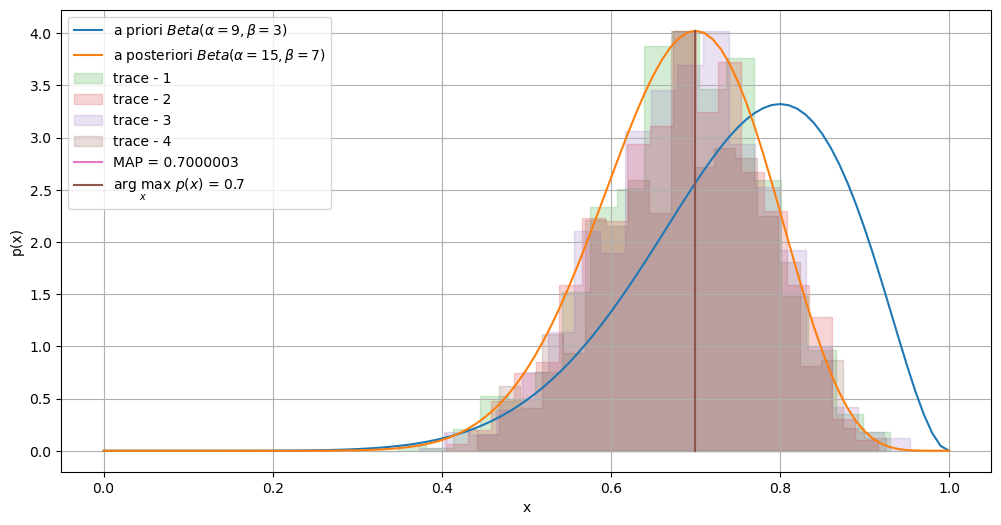
\includegraphics[width=1\textwidth]{plots/beta_prior_to_posterior_mcmc.png}
    \caption{Од \textit{a priori} \(Beta(\alpha=9, \beta=3)\) до \textit{a posteriori} со MCMC и MAP}
    \label{fig:beta_prior_to_posterior_mcmc}
\end{figure}

На слика \ref{fig:beta_prior_to_posterior_mcmc} го рекреираме примерот на фрлање паричка од слика \ref{fig:beta_prior_to_posterior}. За дадено \textit{a priori} верување моделирано со распределба \(Beta(\alpha=9, \beta=3)\) и примерок од 6 настани „се падна петка“ и 4 настани „се падна глава“, креираме 4 траси од по 1000 примероци извлечени од \textit{a posteriori} распределбата (која што аналитички пресметано е \(Beta(\alpha=15, \beta=7)\)). Се забележува дека хистограмите од трасите успешно ја апроксимираат \textit{a posteriori} распределбата \footnote{Висината на хистограмите зависи од бројот на примероци кои ги влечеме од \textit{a posteriori} распределбата. Поточно е да се каже дека соодносот на хистограмите добро го апроксимира соодносот на густините на распределби, а токму тоа нам ни е и потребно. На сликата \ref{fig:beta_prior_to_posterior_mcmc} хистограмите се скалирани за да највисокиот хистограм биде еднаков на најголемата густина на \textit{a posteriori} распределбата пресметана аналитички.}. Дополнително, и разликата на MAP оценувачот со вистинската мода на \textit{a posteriori} распределбата е занемарливо ниска, па доколку не интересира вредноста на параметарот со најголема веројаност, можеме да го употребиме MAP оценувачот.

\subsubsection{Веројатносни програмски јазици}

При решавањето на одредена проблематика, од која било област, на располагање ни стојат повеќе програмски јазици и библиотеките кои се развиени во нивниот еко-систем. Доколку се одлучиме Бајесовото моделирање да го направиме во Python, веројатно ќе се одлучиме и да користиме библиотеки како што се NumPy, SciPy, stats итн. Но, на нас останува да ги имплементираме законите на Бајесовото заклучување, односно начините на пресметка на \textit{a posteriori} законот на распределба, MCMC алгоритмот за влечење примероци од \textit{a posteriori} распределбата итн.

Ваквиот метод на имплементирање, каде што експлицитно му „наредуваме“ на програмскиот код што треба да направи, се нарекува императивен метод на имплементирање. Терминот се употребува и во други области на програмирањето (на пример, во веб програмирањето, креирањето на динамичка HTML содржина со JavaScript се нарекува императивно креирање на динамичка содржина).

Постојат т.н. веројатносни програмски јазици кои спаѓаат во групата на декларативни програмски јазици. Овие јазици се нарекуваат декларативни бидејќи, за разлика од императивните програмски јазици, програмерот „декларира“ како изгледа моделот, а јазикот во „позадина“ ги прави сите пресметки кои се потребни за да се имплементира Бајесовото заклучување. И овој термин се употребува и во други области на програмирањето (на пример, во веб програмирањето, креирањето на динамичка HTML содржина со React се нарекува декларативно креирање на динамичка содржина).

Постојат многу веројатносни програмски јазици, меѓу кои најпознати се Stan \cite{carpenter2017stan}, PyMC \cite{abril2023pymc}, Numpyro \cite{bingham2019pyro, phan2019composable} и Tensorflow Probability \cite{tensorflow2015-whitepaper}. Во овој труд, ние ќе го користиме PyMC.

\begin{lstlisting}[language=Python,caption=Фрлање паричка моделирано во PyMC]
import pymc as pm

model = pm.Model()
with model:
    p = pm.Beta("p", alpha=9, beta=3) # a priori
    X = pm.Bernoulli("X", p=p, observed=data) # likelihood
    # similar, using Binomial distribution
    # X = pm.Binomial(
    #     "X",
    #     n=data.shape[0],
    #     p=p,
    #     observed=data.sum()
    # )

    # a posteriori estimates
    # MAP estimate
    point = pm.find_MAP()

    # MCMC trace
    trace = pm.sample()
\end{lstlisting}

За да ги направи неопходните пресметки временски ефикасно, PyMC гради пресметковен граф. Овој пресметковен граф потоа се компајлира, при што се оптимизира бројот на пресметки кои е потребно да бидат направени. Дополнително, ваквиот пресметковен граф дозволува и лесно да се пресметаат изводи, доколку истите станат потребни. PyMC пресметковниот граф го имплементира во PyTensor \cite{pytensor2022}, што е продолжение на Aesara \cite{T_Willard_Aesara_2023}, што е за возврат базирано на Theano \cite{al2016theano}.

PyMC ни нуди повеќе методи за влечење на примероци од \textit{a posteriori} распределбата, но доколку не прецизираме поинаку, се користи NUTS со \verb|jitter+adapt_diag| методата за наоѓање на почетната вредност. Дополнително, PyMC освен што нуди сопствена имплементација на backend за вршење пресметки, на располагање го нуди и backend-от на NumPyro, backend-от blackjax и backend-от nutpie. Овие backend-и нудат и поддршка за забрзување на графичка картичка, што значително го намалува времето на влечење на примероци од \textit{a posteriori} распределбата.

Девелоперите на PyMC нудат и пакет наречен PyMC Extras \cite{pymcextras2022}, каде што се достапни повеќе експериментални и нецелосно тестирани методи. Една од нив ќе биде искористена во овој труд.

\newpage

\section{Опис на моделот Facebook Prophet}

Facebook Prophet е Бајесов модел развиен од Facebook чија цел е моделирање на бизнис временските серии кое успешно скалира при зголемувањето на бројот на временските серии. Мотивацијата позади развивањето на Facebook Prophet се потешкотиите со кои се соочуваат статистичарите при моделирањето на голем број временски серии со дотогаш постоечките пакети.

Во моделирањето на неколку различни временски серии користејќи автоматизирани методи од пакетот \verb|forecast| во R \cite{hyndman2007automatic, hyndman2024}, тимот на Facebook Prophet забележува дека повеќето од нив неуспешно ги реплицираат карактеристиките на временските серии кои се обидуваат да ги моделираат. Притоа, тимот на Facebook Prophet експериментално покажува дека \verb|auto.arima| неуспешно го моделира трендот на временските серии кога во него постојат промени при крајот на самата временска серија, а сезоналностите воопшто не ги моделира\footnote{Впрочем, авторите на Facebook Prophet \cite{taylor2018forecasting} посочуваат дека ARIMA може да ги моделира сезоналните коваријати за временската серија, но повеќе од сигурно е дека аналитичар без поголемо статистичко познавање на овој модел тоа нема успешно да го стори. Истовремено, и времето на извршување на моделот драстично се зголемува со употребата на овие сезонални коваријати.}. \verb|ets| \cite{hyndman2002state} и \verb|snaive| успешно ја моделираат само неделната сезоналност, а \verb|tbats| \cite{de2011forecasting} неуспешно ја моделира годишната сезоналност.

Тимот на Facebook Prophet забележува две потешкотии со кои се соочува полето на моделирање бизнис временски серии: (1) целосното автоматско моделирање на временските серии е нефлексибилно и не дозволува успешно вклучување на бројни хевристики и претпоставки кои би ни биле корисни, и (2) аналитичарите задолжени за моделирање во поголемите организации имаат експертско знаење за проблемот што го моделираат, но не се доволно обучени во полето на статистиката за таквото експертско знаење успешно да го искористат, па се потпираат на претходно споменатото целосно автоматско моделирање.

Во таа смисла, кога зборуваме за скалирање на поголем број временски серии, кај Facebook Prophet не размислуваме за скалирање во однос на времето на извршување и оптималното искористување на хардверските ресурси кои би ни биле потребни, туку за скалирање во однос на човечките ресурси кои би ни биле потребни и различните типови на бизнис временски серии кои би требало да ги моделираме. Идејата на Facebook Prophet е да обезбеди пакет кој е доволно интуитивен за да и аналитичари кои не се експерти во полето на статистиката можат да го користат (како што тоа го прават со пакетите за целосно автоматско моделирање), но истовремено и доволно флексибилен да имплементира хевристики кои потекнуваат од нивното експертското знаење.

Facebook Prophet скалира во однос на човечки ресурси т.е. е доволно интуитивен за употреба и од луѓе кои не се експерти во полето на статистиката, со тоа што самиот по себе ги опфаќа повеќето карактеристики кои го опишуваат трендот, сезоналноста (периодичноста) и празничната сезоналност кои се јавуваат во бизнис временските серии. Аналитичарот не мора да е запознаен со различните функции кои се користат за моделираат трендот, ниту да има познавање од фуриерови серии и тригонометриско моделирање на периодични функции. Но, истовремено, на аналитичарот му се достапни интерпретабилни хипер-параметри чие што подесување соодветствува на вклучувањето на хевристики од експертското знаење на аналитичарот во моделот.

\subsection{Општа дефиниција на моделот}

Дефиницијата на Facebook Prophet во многу погледи наликува на генерализиран адитивен модел \cite{hastie1987generalized, hastie2017generalized}. Конкретно, тоа значи дека излезот на моделот е сума од неколку различни компоненти/модели кои моделираат одредени карактеристики на временската серија и шум. Уште поконкретно, Facebook Prophet е разградлив модел за временски серии \cite{harvey1990estimation} кој, во својата наједноставна форма, се состои од компонента за тренд, компонента за сезоналност и компонента за празнична сезоналност. Временските серии дефинирани во (\ref{timeseries_def}) Facebook Prophet ги моделира со:

\begin{equation}\label{fbprophet_def}
    y(t) = g(t) + \sum_{i=1}^{n}s_i(t) + h(t) + \epsilon_t
\end{equation}

\(s_i(t)\) се компоненти кои ja моделираат сезоналноста на временската серија дадена во (\ref{seasonalities_def}). Facebook Prophet, без потреба од никакви дополнителни спецификации од страна на аналитичарот, се обидува да измоделира неделна и годишна сезоналност, потпирајќи се на одредени правила за тоа дали има доволно податоци да ги моделира. Дополнителните сезоналности што може да го интересираат аналитичарот треба да се прецизираат преку API-то на Facebook Prophet.

\(h(t)\) е компонента што ja моделира празничната сезоналност на временската серија. Оваа компонента е тривијална и може да се разгледува како специјален случај на \(s_i(t)\) компонентите. Понатаму во овој труд нема да посветуваме внимание на оваа компонента, за да не навлеземе беспотребно во креирање на големи таблици со празници.

\(g(t)\) е компонента што го моделира трендот на временската серија. Во однос на (\ref{timeseries_def}), тренд можеме да дефинираме како необјаснетост (резидуал) што преостанува да се моделира во временската серија откако сме ги моделирале сезоналностите кои ни се од интерес. Facebook Prophet нуди два типа на тренд компоненти: линеарни и логистички. Во овој труд, подробно ќе го разгледаме линеарниот тренд.

Важно е да се напомене и дека адитивната форма во (\ref{fbprophet_def}) не е единствената форма на Facebook Prophet. Во случаи кога очекуваме амплитудата на сезоналностите да се менува зависно од \(t\), Facebook Prophet дозволува да користиме т.н. мултипликативна сезоналност за моделирање. Тогаш, моделот од (\ref{fbprophet_def}) преминува во:

\begin{equation}\label{fbprophet_multiplicative_def}
    y(t) = g(t)(1 + \sum_{i=1}^{n}s_i(t) + h(t)) + \epsilon_t
\end{equation}

Згодната нуспојава на мултипликативната форма во (\ref{fbprophet_multiplicative_def}) е интерпретабилноста на \(s(t)\) и \(h(t)\). Имено, во ваквата форма можеме да кажеме дека, за дадена вредност на \(t\), сезоналноста \(s_i\) го менува трендот за \(100 * s_i(t)\) проценти.

Моделот на Facebook Prophet може и дополнително да се усложни со додавање на нови регресори \(r_i(t)\). Важно е да се напомене дека доколку одлучиме да додадеме нови регресори во моделот, потребно е да ги знаеме нивните вредности не само во примерокот, туку и надвор од него, во хоризонтот за кој што предвидуваме.

Моделот на Facebook Prophet е имплементиран во веројатносниот програмски јазик Stan \cite{carpenter2017stan}. Без дополнително подесување, методата на учење на податоците ја користи методата на \textit{maximum a posteriori} (MAP) оценување на параметрите наместо алгоритмот Маркови Вериги Монте Карло. Притоа, се користи L-BFGS алгоритмот \cite{liu1989limited} за наоѓање на вредноста на MAP поради неговата брзина.

\subsection{Тренд}

\subsubsection{Параметри на тренд компонентата}

Поради дефиницијата на проблемот кој овој труд се обидува да го реши, во претходното поглавје позголдно ни беше трендот да го дефинирме како необјаснетост (резидуал) што преостанува да се моделира во временската серија откако сме ги моделирале сезоналностите кои ни се од интерес. Но, поинтуитивно е да започнеме со објаснување на трендот во временските серии, а подоцна сезоналноста да ја гледаме како периодична необјаснетост (резидуал). Тој пристап го има тимот кој стои зад Facebook Prophet, па и тука ние ќе го искористиме тој пристап за да ги објасниме разните компоненти.

Во својата најосновна форма, Facebook Prophet претпоставува дека трендот е линеарен т.е. дека \(g(t) = kt + m\), каде што \(k\) го моделира растот во временската серија, а \(m\) го моделира пресекот со \(y\)-оската.

Понатаму, Facebook Prophet претпоставува дека овој линеарен тренд се менува во \(S\) временски моменти, па имаме вектор на временски моменти \(\boldsymbol{s} \in \mathbb{R} ^ S\). Овие временски моменти се или точно зададени од корисникот, или пак само нивниот број \(S\) е зададен, а Facebook Prophet ги поставува на еднакво растојание низ времето опфатено од примерокот \footnote{Во просечен случај, промена на трендот во моделот при крајот на примерокот доведува до лоши резултати. Затоа, доколку експлицитно не се наведе, Facebook Prophet ги дели првите 80\% од времето на еднакви интервали на кои ги поставува временските моменти на промена на трендот.} т.е. \(\forall i \in \mathbf{N}, \forall j \in \mathbf{N}, i > 1, j > 1, i \leq S, j \leq S \Rightarrow s_i - s_{i-1} = s_j - s_{j-1}\).

Промената на трендот во овие временски моменти Facebook Prophet ја дефинира како промена во растот на временската серија. Тогаш имаме вектор на промени \(\boldsymbol{\delta} \in \mathbf{R}^S\) каде што \(\delta_i\) е промената во растот на временската серија во временскиот момент \(s_i\). Во пракса, кога примерокот се состои од \(N \in \mathbb{N}\) временски моменти означени со \(t_j, j = 1, ..., N\) и истите се претставени со векторот \(\boldsymbol{t} \in \mathbb{R}^N\), растот на временската серија во овие временски моменти можеме да го дефинираме со вектор \(\boldsymbol{k} \in \mathbb{R}^N\) каде што:

\begin{equation}\label{slope_slow}
k_t = k + \sum_{i=1}^{t>s_i} \delta_i
\end{equation}

Секогаш е временски поефикасно, кога можеме, да ги векторизираме сумите (и сите пресметки кои побаруваат бројни итерации за да се дојде до крајниот резултат). Затоа дефинираме вектор \(\boldsymbol{a}(t) \in \{0, 1\}^S\), во кој \(a_i(t) = 1\) кога \(t\) е временски момент поголем од временскиот момент на промена \(s_i\) т.е.

\begin{equation}\label{vector_a}
    a_i(t) = \begin{cases}
    1 & t > s_i \\
    0 & t \leq s_i
\end{cases}
\end{equation}

Сега, (\ref{slope_slow}) може да се векторизира преку (\ref{vector_a}) во \(k_t = k+\boldsymbol{a}(t)^{\top}\boldsymbol{\delta}\). Конечно, креираме и матрица \(\boldsymbol{A} \in \mathbb{R}^{N \times S}\) која што ни дозволува во еден чекор да ги пресметаме вредностите на векторот \(\boldsymbol{k}\):

\begin{equation}\label{matrix_a}
    \begin{aligned}
        A_{j,i} = a_i(t_j)\\
        \boldsymbol{k} = k + \boldsymbol{A}\boldsymbol{\delta}
    \end{aligned}
\end{equation}

Доколку сакаме линеарниот тренд да е непрекината функција, потребно е во временските моменти на промена да се модифицира и пресекот со \(y\)-оската. Нека пресекот со \(y\)-оската во различните временски моменти на промена \(s_1, ..., s_S\) се модифицира во \(n_1, ..., n_S\) соодветно. Тогаш, линеарниот тренд можеме да го запишеме како функција на делови:

\begin{equation}\label{piecewise_trend_no_intercept}
g(t) =
    \begin{cases}
        kt + m & t < s_1 \\
        (k + \delta_1)t + n_1 & t \in [s_1, s_2)\\
        ...\\
        (k + \sum_{j=1}^{i}\delta_j)t + n_i & t \in [s_i, s_{i+1})\\
        ...\\
        (k + \sum_{j=1}^{S}\delta_j)t + n_S & t \geq s_S
    \end{cases}
\end{equation}

(\ref{piecewise_trend_no_intercept}) е непрекината функција ако и само ако за секој временски момент на промена \(s_i, i > 1\) важи:

\begin{equation}\label{intercept_connection}
(k + \sum_{j=1}^{i - 1}\delta_j)s_i + n_{i-1} = (k + \sum_{j=1}^{i}\delta_j)s_i + n_i \Rightarrow n_i = n_{i-1} - \delta_is_i
\end{equation}

Во специјалниот случај кога временскиот момент на промена е \(s_1\), (\ref{piecewise_trend_no_intercept}) е непрекината функција ако и само ако:

\begin{equation}\label{intercept_trivial}
ks_1 + m = (k + \delta_1)s_1 + n_1 \Rightarrow n_1 = m - \delta_1s_1
\end{equation}

Почнувајќи со (\ref{intercept_trivial}) и рекурзивно применувајќи го (\ref{intercept_connection}) добиваме вредности за \(n_i\):

\begin{equation}\label{intercept_sum}
    n_i = m - \sum_{j=1}^{i} \delta_js_j
\end{equation}

Во примерокот од \(N\) временски моменти, пресекот со \(y\)-оската можеме да го дефинираме со вектор \(\boldsymbol{m} \in \mathbb{R}^N\), па од (\ref{intercept_sum}) се добива:

\begin{equation}\label{intercept_final}
    \begin{gathered}
        m_i = m - \sum_{i=1}^{t>s_i} \delta_is_i = m - \boldsymbol{a}(t)^{\top}(\boldsymbol{\delta}\odot\boldsymbol{s}) \\
        \boldsymbol{m} = m - \boldsymbol{A}(\boldsymbol{\delta}\odot\boldsymbol{s})
    \end{gathered}
\end{equation}

Конечно, тренд компонентата можеме да ја запишеме како:

\begin{equation}\label{trend_final_func}
    g(t) = (k + \boldsymbol{a}(t)^{\top}\boldsymbol{\delta}) + (m - \boldsymbol{a}(t)^{\top}(\boldsymbol{\delta}\odot\boldsymbol{s}))
\end{equation}

Во примерокот од \(N\) временски моменти,  вредноста на трендот можеме да ја дефинираме со вектор \(\boldsymbol{g} \in \mathbb{R}^N\), па од (\ref{matrix_a}), (\ref{intercept_final}) и (\ref{trend_final_func}) се добива:

\begin{equation}\label{trend_final_vectorized}
    \begin{aligned}
        \boldsymbol{g} & = \boldsymbol{k} \odot \boldsymbol{t} + \boldsymbol{m} \\
        &=(k + \boldsymbol{A}\boldsymbol{\delta}) \odot \boldsymbol{t} + m - \boldsymbol{A}(\boldsymbol{\delta}\odot\boldsymbol{s})
    \end{aligned}
\end{equation}

\subsubsection{Моделирање на \textit{a priori} распределбата на параметрите во тренд компонентата}

Од (\ref{trend_final_vectorized}) забележуваме дека имаме три недетерминистички параметри кои можеме да ги моделираме со \textit{a priori} закони на распределба:

\begin{itemize}
    \item \(k\) е иницијалниот раст на трендот. Користиме нормална \textit{a priori} распределба со параметри \(\mu = 0\) и \(\sigma = 5\). Поголема вредност на \(\sigma\) ја зголемува флексибилноста на растот на трендот да се прилагоди на примерокот и да отстапи од \(\mu\) и, обратно, помала вредност на \(\sigma\) ја зголемува пристрасноста на растот на трендот да биде блиску до \(\mu\).
    \item \(m\) е иницијалниот пресек на трендот со \(y\)-оската. Слично на \(k\), користиме нормална \textit{a priori} распределба со параметри \(\mu = 0\) и \(\sigma = 5\). Повторно важи дека поголема вредност на \(\sigma\) ја зголемува флексибилноста на пресекот на трендот со \(y\)-оската да се прилагоди на примерокот и да отстапи од \(\mu\) и, обратно, помала вредност на \(\sigma\) ја зголемува пристрасноста на пресекот на трендот со \(y\)-оската да биде блиску до \(\mu\).
    \item \(\boldsymbol{\delta}\) е вектор на промени на растот на трендот. Во пракса прецизираме поголем број на временски моменти каде што може да настане промена на растот на трендот, но самите промени ги моделираме со \textit{a priori} распределба која што е проретчена т.е. има висока густина на распределба околу нулата, со цел повеќето промени да се блиску до нулата. Користиме двојно експоненцијална т.е. Лапласова \textit{a priori} распределба со параметри \(\mu = 0\) и \(\tau = 0.05\). Поголема вредност на \(\tau\) резултира со помал степен на проретченост т.е. поголем број на промени на растот на трендот т.е. поголема флексибилноста на трендот да се прилагоди на примерокот и, обратно, помала вредност на \(\tau\) резултира со повисок степен на проретченост т.е. ја зголемува пристрасноста на трендот да го задржи иницијалниот раст (да биде линеарен тренд, наместо линеарен тренд искршен да делови).
\end{itemize}

Во имплементацијата на Ritchie Vink на Facebook Prophet во PyMC3 \cite{vink} се наведува дека изборот на \(\tau = 0.05\) е премногу пристрасен кон мал број на промени на растот на трендот. Затоа, дополнително и параметарот \(\tau\) на двојно експоненцијалниот \textit{a priori} закон на распределба на \(\boldsymbol{\delta}\) е моделиран со сопствен експоненцијален \textit{a priori} закон на распределба со параметар \(\lambda = 1.5\). Помала вредност на \(\lambda\) резултира со помал степен на проретченост \footnote{Очекувањето на експоненцијалната распределба е \(\frac{1}{\lambda}\), па помала вредност на \(\lambda\) резултира со повисоко очекување.} т.е. поголем број на промени на растот на трендот т.е. поголема флексибилноста на трендот да се прилагоди на податочното множество и, обратно, поголема вредност на \(\lambda\) резултира со повисок степен на проретченост т.е. ја зголемува пристрасноста на трендот да го задржи иницијалниот раст (да биде линеарен тренд, наместо линеарен тренд искршен да делови).

\subsubsection{Несигурност во тренд компонентата}

Facebook Prophet не поставува временски моменти на промена на растот на трендот кога истиот го пресметува надвор од примерокот, туку задржува константна стапка на раст. За проценка на несигурноста на трендот, претпоставуваме дека во секој временски момент надвор од примерокот може да настане промена на растот на трендот со иста честота и магнитуда како и внатре во примерокот.

Магнитудата на промената на растот на трендот надвор од примерокот ја моделираме со \(\delta_i \sim Laplace(0, \tau)\), каде што \(\tau\) можеме да го моделираме или како хиерархиски приор (како што беше споменато во претходното поглавје за имплементацијата на Ritchie Vink \cite{vink}), или пак можеме да го оцениме со оценувач на максимална подобност така што \(\widehat{\tau} = \frac{1}{S}\sum_{i=1}^{S}|\delta_i|\). Во тој случај, за секој временски момент \(t\) надвор од примерокот имаме промена на растот на трендот \(\delta_t\) која го следи законот на распределба:

\begin{equation}\label{trend_uncertainty}
P(\delta_t=x) =
    \begin{cases}
        \frac{N - S}{N} & x=0 \\
        \hfil \frac{S}{T}, & x \sim Laplace(0, \frac{1}{S}\sum_{i=1}^{S}|\delta_i|)
    \end{cases}
\end{equation}

\subsection{Сезоналност}

\subsubsection{Параметри во сезоналната компонента}

Во Facebook Prophet, сезоналноста се моделира со Фуриеров ред \cite{harvey199310}. За дадена периода \(P\) сезоналноста ја моделираме со \(C\) компоненти:

\begin{equation}\label{fourier_seasonality}
\begin{aligned}
    s(t) &= \sum_{i=1}^{C} (a_ncos(\frac{2\pi it}{P}) + b_nsin(\frac{2\pi it}{P})) \\
    &= [cos(\frac{2\pi t}{P}), sin(\frac{2\pi t}{P}), ..., cos(\frac{2\pi Ct}{P}), sin(\frac{2\pi Ct}{P})][a_1,b_1,...,a_C,b_C]^T \\
    &= X(t)\boldsymbol{\beta}
\end{aligned}
\end{equation}

Изборот на бројот на компоненти \(C\) влијае на флексибилноста на компонентата да се прилагоди на примерокот т.е. повисока вредност на \(C\) придонесува до сезоналност која што има поголема флексибилност да се прилагоди на примерокот, а пониска вредност на \(C\) придонесува до поедноставна сезоналност. Во пракса, Facebook Prophet заклучиле дека е сосема доволно за \(P=365.25\) (годишна сезоналност) да се користат \(C=10\) компоненти, а за \(P=7\) (неделна сезоналност) да се користат \(C=3\) компоненти.

\subsubsection{Моделирање на \textit{a priori} распределбата на параметрите во сезоналната компонентата}

Од \ref{fourier_seasonality} забележуваме дека имаме еден недетерминистички параметар кој можеме да го моделираме со \textit{a priori} закон на распределба. \boldsymbol{\beta} е вектор на коефициенти на тригонометрискиот ред. Користиме нормална \textit{a priori} распределба со параметри \(\mu=0\) и \(\sigma=10\). Повисока вредност на \(\sigma\), слично како и повисоката вредност на бројот на компоненти \(C\) ја зголемува флексибилноста на сезоналноста да се прилагоди на примерокот.

\subsection{Пред-процесирање на примерокот}

Facebook Prophet прави многу едноставно пред-процесирање на примерокот. За самиот пристап на моделирање опишан во претходните неколку подглавја не е важно дали во примерокот има вредности кои недостигаат, ниту пак дали постојат outliers.

Единственото пред-процесирање на вредностите на временската серија што се применува е скалирањето. Facebook Prophet нуди два типа на скалирање на примерокот \(\{X_{1}, ..., X_{N}\}\):
\begin{itemize}
    \item \verb|absmax| скалирање, каде што примерокот се скалира делејќи ја вредноста во секој временски момент со максималната апсолутна вредност во временската серија т.е. \(X_{i}=\frac{X_{i}}{max\{|X_{1}|, ..., |X_{N}|\}}\)
    \item \verb|minmax| скалирање, каде што примерокот се скалира линеарно помеѓу 0 и 1 т.е. \(X_{i}=\frac{X_{i} - min\{X_{1}, ..., X_{N}\}}{max\{X_{1}, ..., X_{N}\} - min\{X_{1}, ..., X_{N}\}}\)
\end{itemize}

Временските моменти секогаш се скалираат со \verb|minmax| скалирање, така што првиот елемент во примерокот се случува во временски момент 0, а последниот во временски момент 1 т.е. \(t_{i}=\frac{t_{i} - min\{t_{1}, ..., t_{N}\}}{max\{t_{1}, ..., t_{N}\} - min\{t_{1}, ..., t_{N}\}}\).

\subsection{Почетни вредности}

Изборот на почетни вредности за сезоналната компонента е тривијален - едноставно, ги поставуваме сите почетни вредности за коефициентите \(\boldsymbol{\beta}\) на 0. Истиот принцип го применуваме и за векторот на промени на растот на трендот \(\boldsymbol{\delta}\).

Изборот на почетна вредност за иницијалниот раст на трендот \(k\) е поспецифична. За да можат алгоритмите MCMC и L-BFGS да работат ефикасно, избираме почетна вредност за \(k\) претпоставувајќи дека нема да има ниту еден временски момент на промена на растот на трендот (оваа претпоставка соодветствува на изборот на почетна вредност на \(\boldsymbol{\delta}\) што го направивме). Под ваква претпоставка, почетна вредност за \(k\) ја избираме така што да соодветствува на растот на линијата што ги поврзува вредностите на временската серија во најраниот и најдоцниот временски момент т.е.

\begin{equation}\label{init_slope}
    k_{init} = \frac{X_{argmax\{\boldsymbol{t}\}} - X_{argmin\{\boldsymbol{t}\}}}{max\{\boldsymbol{t}\}-min\{\boldsymbol{t}\}}
\end{equation}

Соодветниот пресек со \(y\)-оската е добра почетна вредност за параметарот \(m\), па од (\ref{init_slope}) следи:

\begin{equation}\label{init_intercept}
    m_{init} = X_{argmin\{\boldsymbol{t}\}}-min\{\boldsymbol{t}\}*k_{init}
\end{equation}

\subsection{Опис на интерфејсот} \label{prophet_api}

Facebook Prophet ја следи т.н. парадигма на „течен интерфејс“ \cite{fowler2005fluent}. Во пракса, тоа значи дека секој метод што ја менува формата на моделот за повратна вредност ја има новата форма на моделот. Во кодот подоле дефинираме модел во Facebook Prophet кој што ќе ја има формата \(y(t) = g(t)(1 + s_1(t) + s_2(t) + s_3(t)) + \epsilon_t\) каде што \(s_1(t)\) е годишна сезоналност со периода од 365.25 претставена преку 10 фуриерови компоненти, \(s_2(t)\) е месечна сезоналност со периода од 30.5 претставена преку 5 фуриерови компоненти и \(s_3(t)\) е неделна сезоналност со периода од 7 претставена преку 3 фуриерови компоненти.

\begin{lstlisting}[language=Python,caption=Дефинирање на Facebook Prophet модел]
model = Prophet(
    seasonality_mode="multiplicative",
    yearly_seasonality=10,
    weekly_seasonality=3,
).add_seasonality(
    name="monthly",
    period=30.5,
    fourier_order=5,
)
\end{lstlisting}

Се забележува дека во самото инстанцирање на објект од класата \verb|Prophet| ние го наведуваме бројот на фуриерови компоненти кои сакаме да ги користиме за моделирање на годишната и неделната сезоналност. Но, додавањето на месечната сезоналност се прави со повикување на метод \verb|add_seasonality| кој како повратна вредност го има модифицираниот објект, каде што месечната сезоналност е додадена.

Ваквиот интерфејс не ограничува во дефинирањето на моделите, или ја намалува читкоста и интуитивноста на програмскиот код. Доколку посакавме да дефинираме модел користејќи ги истите сезоналности како и претходно, но овојпат со формата \(y(t)=g(t)s_1(t)(1 + s_2(t)) + s_3(t) + \epsilon_t\), во која мешаме различни методи на додавање на сезоналност (\(s_1\) е обична мултипликативна сезоналност, \(s_2\) е покомплицирана мултипликативна сезоналност и \(s_3\) е адитивна сезоналност), ова немаше да можеме да го сториме. Во најдобар случај ќе можевме да дефинираме модел со форма \(y(t)=g(t)(1 + s_1(t) + s_2(t)) + s_3(t) + \epsilon_t\) со многу неинтуитивен програмски код.

\begin{lstlisting}[language=Python,caption=Дефинирање на покомплексен Facebook Prophet модел]
model = Prophet(
    seasonality_mode="multiplicative",
    yearly_seasonality=10,
    weekly_seasonality=False,
).add_seasonality(
    name="monthly",
    period=30.5,
    fourier_order=5,
    mode="multiplicative",
).add_seasonality(
    name="weekly",
    period=7,
    fourier_order=3,
    mode="additive",
)
\end{lstlisting}

\newpage

\section{Опис на моделот базиран на Facebook Prophet - Vangja}

Vangja е пакет направен во програмскиот јазик Python. Целта на Vangja беше да обезбеди пакет за креирање модели инспирирани од моделите користени во Facebook Prophet кои ќе можат да „научат“ сезонални карактеристики на временски серии од кои поседуваме поголем примерок и истите да ги „модифицираат“ за моделирање на сезонални карактеристики на временски серии од кои поседуваме помал примерок.

Мотивацијата за Vangja потекна од потешкотиите кои ги имавме во обидот да го прилагодиме Facebook Prophet на проблемот кој што сакавме да го решиме (и кој е подробно опишан во подглавјето \ref{problem_definition}). Интерфејсот на Facebook Prophet (опишан во подглавјето \ref{prophet_api}) не ни дозволуваше да додадеме нови компоненти при моделирањето на временските серии, а постоечките компоненти не беа лесни за адаптирање на идеите кои сакавме да ги примениме.

Од друга страна, постоечкиот пакет \verb|TimeSeers| \cite{timeseers2021} ја нудеше флексибилност што ја баравме, но авторот не го одржуваше проектот, кој и самиот беше имплементиран во застарена верзија на PyMC. Затоа се решивме да креираме пакет кој што ќе го понуди флексибилниот интерфејс на пакетот \verb|TimeSeers|, ќе биде имплементиран во најновата верзија на PyMC и ќе понуди имплементација на идеите кои заземаат централно место во овој труд.

При реимплементација на компонентите на Facebook Prophet во PyMC, освен од пакетот \verb|TimeSeers|, инспирација влечевме и од имплементацијата на Ritchie Vink на Facebook Prophet во PyMC3 \cite{vink}, имплементацијата на \verb|PM-Prophet| \cite{pmprophet2020} во PyMC3 и туторијалот на PyMC за мултипликативна сезоналност во Facebook Prophet \cite{airpassengers}.

\subsection{Интуитивно API и флексибилност}

\subsection{Аналогија со .fit и .tune од deep learning}

\subsection{Различни начини на употреба на \textit{a posteriori} распределбата на сезоналноста од долгата временска серија како \textit{a priori} распределба на сезоналноста на кратката временска серија}

\subsubsection{Наивен пристап}

\subsubsection{Околински пристап}

\subsubsection{Линеарна модификација}

\subsubsection{Контра-сезоналност}

\newpage

\section{Методологија}

\subsection{Податочно множество}

\subsection{Дефинирање различни модели}

\subsection{Краток осврт за хипер-параметрите}

\subsection{Поделба на тренирачко, валидациско и тестирачко множество}

\subsection{Опис на метрики}

\subsection{Експерименти}

\newpage

\section{Заклчуок}

\newpage

\section{Понатамошна работа}

\newpage

\listoffigures

\newpage

\lstlistoflistings

\newpage

\bibliographystyle{abbrv}
\bibliography{sample}

\end{document}
